\subsection{Виртуальное моделирование системы}
Описанная система была смоделирована в среде Unity, её внешний вид представлен на рисунке \ref{pic:unity_model}. Мир 
Unity предназначен для базовой проверки работоспособности испытываемого принципа, поэтому не содержит подробной модели
какого-либо робота. В нём присутствуют: плоскость земли, кронштейн, на котором сверхширокоугольные камеры закреплены под углом $90\deg$, 
и различные объекты-цели, предназначенные для оценки расстояния. В силу особенностей работы многих алгоритмов стереозрения
эти объекты должны сильнотекстурированы \cite{}. % TODO: вставить ссылку на обзор алгоритмов 
\begin{figure}[H]
    \begin{center}
        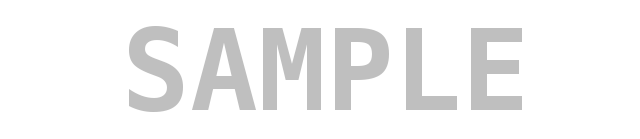
\includegraphics[scale=0.5]{pics/sample.png}                                                                                            %TODO: перерисовать схему?
        \caption{Внешний вид модели системы стереозрения}
        \label{pic:unity_model}
    \end{center}
\end{figure}
В Unity создание сцены происходит с использованием встроенных примитивов, импортированных файлов моделей популярных форматов
или моделей из магазина ассетов, предлагающего обширную библиотеку объектов и текстур, повторяющих различные реальные объекты. В данной 
работе использовались как и примитивы для создания простых объектов, так и модели из магазина для имитации препятствий и окружения.

Для моделирования камеры "рыбий глаз" использовался аддон Dome Tools из магазина Unity Asset Store.    % TODO: проверить все названия
Он позволяет моделировать сверхширокоугольные объективы с разным углом зрения в эквидистантной проекции \cite{}. % TODO: тут бы сослаться на их работку какую-нибудь
При этом с точки зрения других искажений, не относящихся к моделированию правильной проекции, снимки с этой камеры получаются идеальными. % FIXME: моделированию чего? 
Окно настроек камеры представлено на рисунке \ref{pic:camera_settings}.
\begin{figure}[H]
    \begin{center}
        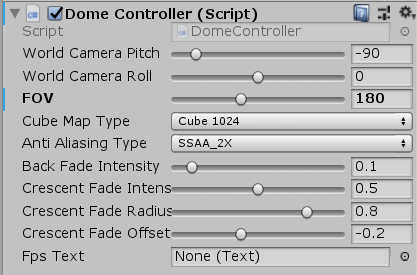
\includegraphics[scale=0.5]{pics/camera_settings.png}                                                                                            %TODO: перерисовать схему?
        \caption{Окно настроек виртуальной камеры в Unity}
        \label{pic:camera_settings}
    \end{center}
\end{figure}
Для виртуальной камеры доступны настройки угла зрения и виньетки по краям изображения,  % FIXME: виньетки -> абберации ??
а также различных параметров рендеринга, влияющих на качество получаемого изображения. 